\subsubsection{Man in the Middle (MITM)}
\label{mitm-sec}
The man in the middle attack puts the attacker between the station and the access point, allowing them to eavesdrop on communications taking place. In wireless communications, monitoring passing traffic is made possible, with the correct setup, as traffic is broadcast and picked up by all network cards in the vicinity; but usually discarded if not intended recipient. Whilst this is a complex process, libraries and software have been created to allow those with a good background knowledge to create MITM exploits. This attack potentially gives the attacker access to user data sent over unencrypted protocols such as HTTP, but also allows them to use tools such as sslstrip \cite{research:ssl_strip} to attempt to thwart HTTPS.

\begin{figure}[h!]
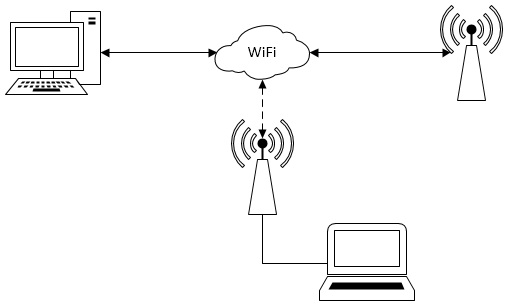
\includegraphics[width=\linewidth]{research/figures/mitm.png}
\caption{Malicious user monitors and injects data packets in to traffic.}
\end{figure}

This style of attack is a popular choice when communications involve some type of public key encryption. 

A more recent variation to this attack, that reflects the shift toward web applications, is the Man in the Browser\footnote{The Boy in the Browser attack \cite{research:bitb} is a less mature version of the Man in the Browser attack. It is a trojan that routes traffic to the attacker’s proxy website to modify before sending to the intended destination.} (MitB). The advantage this has over the vanilla MITM attack is SSL style authentication measures do not hinder its effectiveness. Examples of the MitB attack include HTTP Cache Poisoning \cite{research:cache_poisoning} and HTTP Response Splitting \cite{research:response_splitting}, both can leave lasting effects on the compromised browser.

%This attack will feature in the project implementation as a means of inspecting leaked data from applications when stations are caught in the honeypot.